% ||||||||||||||||||||||||||||||||||||||||||||||
% Arquivo de apresentação
% ||||||||||||||||||||||||||||||||||||||||||||||

\documentclass[aspectratio=169]{beamer}
\mode<presentation>
{
	\usetheme{Madrid}
    
    \definecolor{unisinos}{RGB}{32,64,154}
    \usecolortheme[named=unisinos]{structure}
    
	\usefonttheme{professionalfonts}
    \usebackgroundtemplate{
\includegraphics[width=\paperwidth,height=0.978\paperheight]{template_unisinos}}

 	\beamertemplatenavigationsymbolsempty
 	\setbeamertemplate{footline}
	{
	  \leavevmode%
	  \hbox{%
	  \begin{beamercolorbox}[wd=.12\paperwidth,ht=2.25ex,dp=1ex,center]{author in head/foot}%
	    \usebeamerfont{author in head/foot}\insertshortauthor
	  \end{beamercolorbox}%
	  \begin{beamercolorbox}[wd=.88\paperwidth,ht=2.25ex,dp=1ex,center]{title in head/foot}%
	    \usebeamerfont{title in head/foot}\insertshorttitle\hspace*{3em}
	    \insertframenumber{} / \inserttotalframenumber\hspace*{1ex}
	  \end{beamercolorbox}}%
	  \vskip0pt%
	}
 	\setbeamertemplate{caption}[numbered]
 	\usepackage{caption}

 	\usepackage[brazil]{babel}		% Idioma do documento
	\usepackage{siunitx}
	\usepackage{ragged2e}
	\usepackage{float}
    \usepackage{indentfirst} }
    \usepackage[alf]{abntex2cite}		% Citações padrão ABNT
	\usepackage{color}			% Controle das cores
	\usepackage[T1]{fontenc}		% Selecao de codigos de fonte.
	\usepackage{graphicx}			% Inclusão de gráficos
	\usepackage[utf8]{inputenc}		% Codificacao do documento (conversão automática dos acentos)
	\usepackage{txfonts}			% Fontes virtuais

\title[ Detecção e Diagnóstico Automático de Falhas em Motores Elétricos de Indução via Análise de Assinaturas na
Corrente Elétrica Utilizando ...]
{Detecção e Diagnóstico Automático de Falhas em Motores Elétricos de Indução via Análise de Assinaturas na
Corrente Elétrica Utilizando Técnicas de Clusterização}
\author[Piaia, G. A.]{
	{\fontsize{10}{8}\selectfont \textbf{Mestrando:} Guilherme Angelo Piaia} \\
	{\fontsize{10}{8}\selectfont \textbf{Orientador:} Prof. Dr. Rodrigo Marques de Figueiredo}
}
%\institute[UNISINOS]{UNISINOS - Universidade do Vale do Rio dos Sinos \\ Engenharia de Controle e Automação}

\date{\today}

\begin{document}

%%%%%%%%%%%%%%%%%%%%%%%%%%%%%%%%%%%

\begin{frame}
	\begin{minipage}{1\linewidth}
		\centering
		    \textbf{UNIVERSIDADE DO VALE DO RIO DOS SINOS - UNISINOS} \\ UNIDADE ACADÊMICA DE PESQUISA E PÓS-GRADUAÇÃO \\ PROGRAMA DE PÓS-GRADUAÇÃO EM ENGENHARIA ELÉTRICA \\ NÍVEL MESTRADO PROFISSIONAL
	\end{minipage}
	\titlepage
\end{frame}

%%%%%%%%%%%%%%%%%%%%%%%%%%%%%%%%%%%

\begin{frame}{Sumário}
	\tableofcontents
\end{frame}

%%%%%%%%%%%%%%%%%%%%%%%%%%%%%%%%%%%

\section{Introdução}
\begin{frame}{Introdução}
	\begin{itemize}
		\justifying
		\item Uma das formas de se controlar a posição de um satélite é através da variação do momento angular de rodas.
		\item Diversas técnicas de controle são empregadas para se controlar essa posição. O tipo mais usado é o controlador PID  (Proporcional-Integral-Derivativo).
		\item Este trabalho tem por principal objetivo a implementação em um sistema embarcado
de um controlador com sintonia automática utilizando conceitos de controle inteligente e testa-lo em um simulador de satélites com rodas de reação.
    \end{itemize}
\end{frame}

%%%%%%%%%%%%%%%%%%%%%%%%%%%%%%%%%%%

\begin{frame}{Referencial Teórico - Motores Elétricos de Inclusão}
	\begin{columns}
    	\begin{column}{0.50\textwidth}
			\begin{figure}[HT]
				\begin{center}
					\captionsetup{justification=justified}
					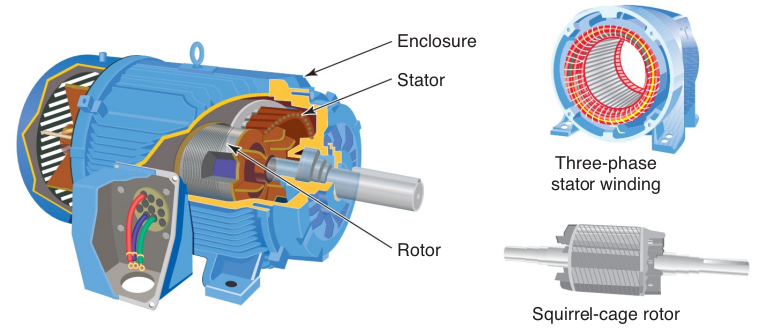
\includegraphics[scale=.3]{../referencial/img/ind_motor_petruzella_p115.png}
					\caption{Motor elétrico de indução tipo gaiola de esquilo. \newline
					Fonte: \citeonline{Petruzella1911}.}
					\label{fig:ind_motor_petruzella_p115}
				\end{center}
			\end{figure}
     	\end{column}
		
		\begin{column}{0.5\textwidth}
			\begin{itemize}
				\item infos
			\end{itemize}
	 	\end{column}
	 \end{columns}
\end{frame}

%%%%%%%%%%%%%%%%%%%%%%%%%%%%%%%%%%%

\begin{frame}{Referencial Teórico - Motores Elétricos de Inclusão}
	\begin{columns}
    	\begin{column}{0.50\textwidth}
			\begin{figure}[HT]
				\begin{center}
					\captionsetup{justification=justified}
					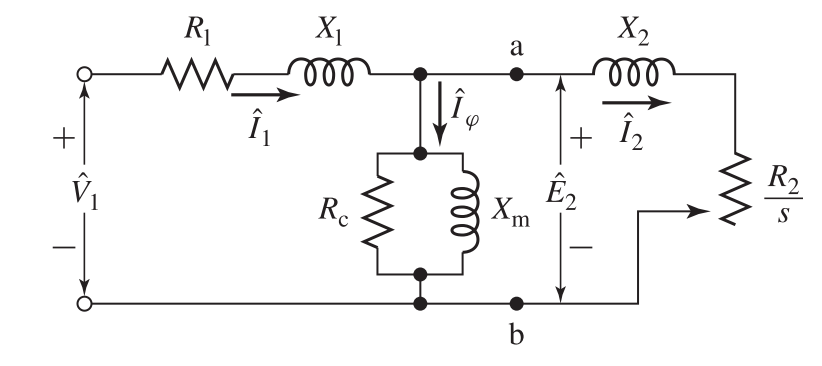
\includegraphics[scale=.25]{../referencial/img/circuit_fitzgerald_p354.png}
					\caption{Circuito equivalente monofásico de um motor de indução polifásico. \newline
					Fonte: \citeonline{Umans2003}.} 
					\label{fig:circuit_fitzgerald_p354}
				\end{center}
			\end{figure}
     	\end{column}
		
		\begin{column}{0.5\textwidth}
			\begin{itemize}
				\item infos
			\end{itemize}
	 	\end{column}
	 \end{columns}
\end{frame}

%%%%%%%%%%%%%%%%%%%%%%%%%%%%%%%%%%%

\begin{frame}{Referencial Teórico - Falhas em Motores Elétricos de Indução}
	\begin{columns}
    	\begin{column}{0.50\textwidth}
			\begin{figure}[HT]
				\begin{center}
					\captionsetup{justification=justified}
					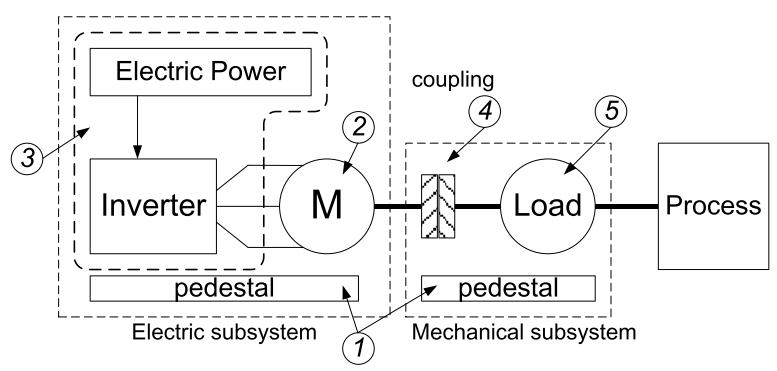
\includegraphics[scale=.25]{../referencial/img/motor_system_rilski_p2.png}
					\caption{Visão geral de sistema com um motor elétrico. \newline
					Fonte: \citeonline{Gorbounov2018}.} 
					\label{fig:motor_system_rilski_p2}
				\end{center}
			\end{figure}
     	\end{column}
		
		\begin{column}{0.5\textwidth}
			\begin{figure}[HT]
				\begin{center}
					\captionsetup{justification=justified}
					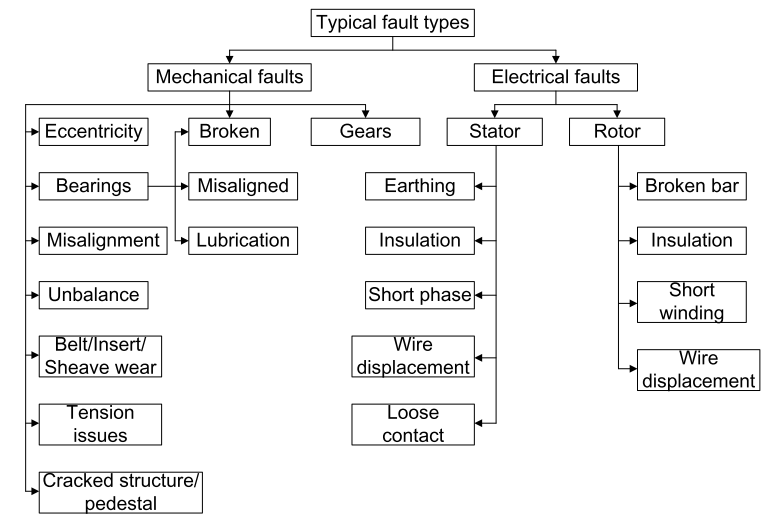
\includegraphics[scale=.27]{../referencial/img/faults_rilski_p77.png}
					\caption{Árvore dos principais tipos de \newline
					falhas em motores elétricos. \newline
					Fonte: \citeonline{Gorbounov2018}.} 
					\label{fig:faults_rilski_p77}
				\end{center}
			\end{figure}
	 	\end{column}
	 \end{columns}
\end{frame}

%%%%%%%%%%%%%%%%%%%%%%%%%%%%%%%%%%%

\begin{frame}{Referencial Teórico - Falhas em Motores Elétricos de Indução}
	\begin{columns}
    	\begin{column}{0.50\textwidth}
			\begin{figure}[HT]
				\begin{center}
					\captionsetup{justification=justified}
					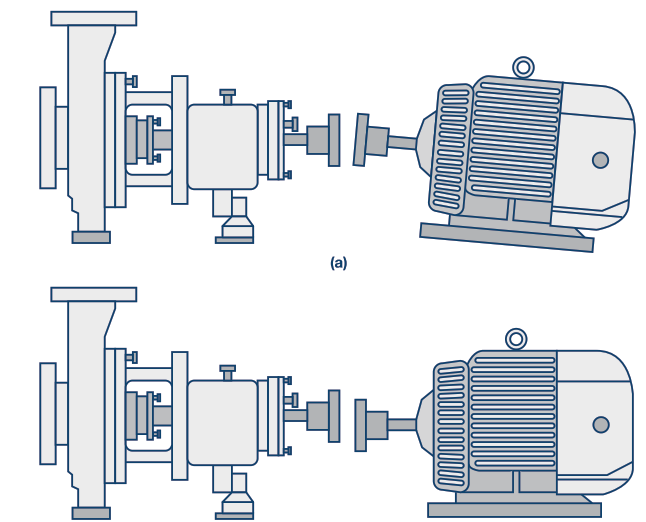
\includegraphics[scale=.25]{../referencial/img/misadraw_analog_p2.png}
					\caption{Ilustração com os tipos de desalinhamento. \newline
					Fonte: \citeonline{Sopcik2019}.} 
					\label{fig:misadraw_analog_p2}
				\end{center}
			\end{figure}
     	\end{column}
		
		\begin{column}{0.5\textwidth}
			\begin{figure}[HT]
				\begin{center}
					\captionsetup{justification=justified}
					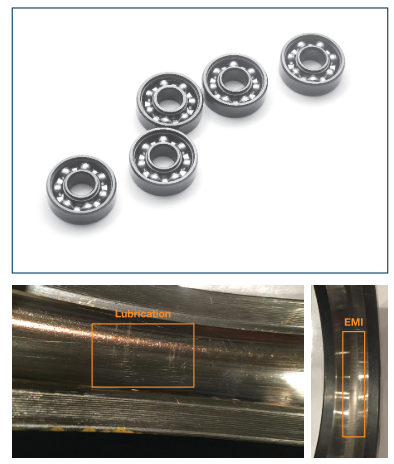
\includegraphics[scale=.3]{../referencial/img/bearing_analog_p3.png}
					\caption{Imagens de rolamentos no \newline
					topo, e falhas na parte de baixo. \newline
					Fonte: \citeonline{Sopcik2019}.} 
					\label{fig:faults_rilski_p77}
				\end{center}
			\end{figure}
	 	\end{column}
	 \end{columns}
\end{frame}

%%%%%%%%%%%%%%%%%%%%%%%%%%%%%%%%%%%

\begin{frame}{Referencial Teórico - Análise de Vibração}
	\begin{columns}
    	\begin{column}{0.50\textwidth}
			\begin{figure}[HT]
				\begin{center}
					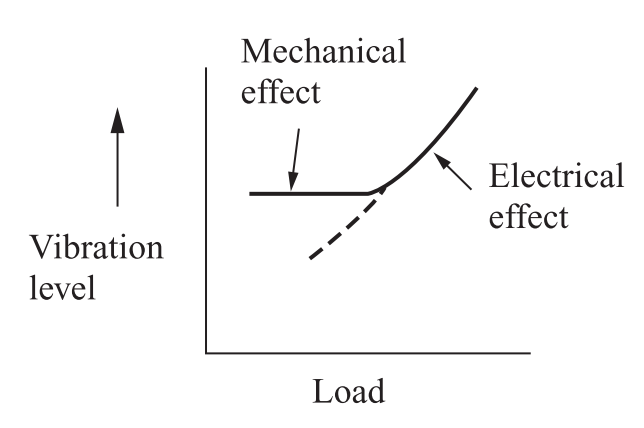
\includegraphics[scale=.25]{../referencial/img/fault_effect_randall_p54.png}
					\caption{Variação da carga para distinção da causa do efeito observado. \newline
					Fonte: \citeonline{Wu2013}.} 
					\label{fig:fault_effect_randall_p54}
				\end{center}
			\end{figure}
     	\end{column}
		
		\begin{column}{0.5\textwidth}
			\begin{itemize}
				\item Infos
			\end{itemize}
	 	\end{column}
	 \end{columns}
\end{frame}

%%%%%%%%%%%%%%%%%%%%%%%%%%%%%%%%%%%

\begin{frame}{Referencial Teórico - Análise de Vibração}
	\begin{columns}
    	\begin{column}{0.50\textwidth}
			\begin{figure}[HT]
				\begin{center}
					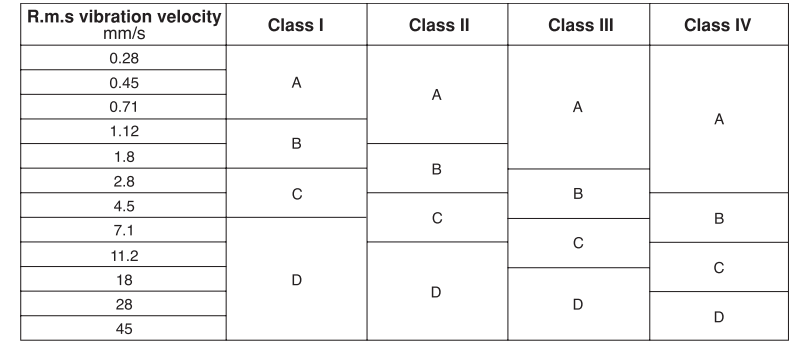
\includegraphics[scale=.28]{../referencial/img/iso10816-1_randall_p146.png}
					\caption{Tabela de valores eficaz máximos de velocidade para cada porte de máquina indicados pela norma ISO 10816-1. \newline
					Fonte: \citeonline{Wu2013}.} 
					\label{fig:iso10816-1_randall_p146}
				\end{center}
			\end{figure}
     	\end{column}
		
		\begin{column}{0.5\textwidth}
			\begin{itemize}
				\item A = bom estado
				\item B = aceitável
				\item C = apenas tolerável
				\item D = não permitido
				\item Classe I = pequenas máquinas (potência menor que $\SI{15}{\kilo\watt}$)
				\item Classe II = máquinas médias sem uma fundação especial (potência entre $\SI{15}{\kilo\watt}$ e $\SI{75}{\kilo\watt}$)
				\item Classe III = máquinas grandes sobre uma fundação rígida e pesada
				\item Classe IV = máquinas grandes \newline
				sobre uma fundação flexível (turbomáquinas) 
			\end{itemize}			
	 	\end{column}
	 \end{columns}
\end{frame}

%%%%%%%%%%%%%%%%%%%%%%%%%%%%%%%%%%%

\begin{frame}{Referencial Teórico - Análise de Vibração}
	\begin{columns}
    	\begin{column}{0.50\textwidth}
			\begin{figure}[HT]
				\begin{center}
					\captionsetup{justification=justified}
					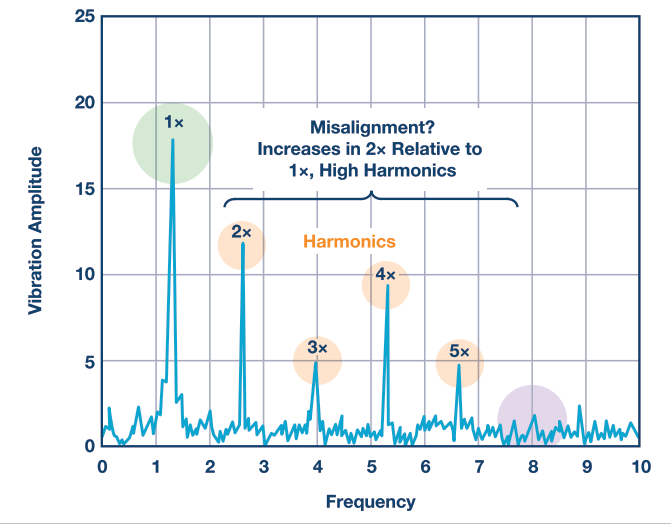
\includegraphics[scale=.25]{../referencial/img/misa_analog_p2.png}
					\caption{Indicação espectral de desalinhamento na velocidade. \newline
					Fonte: \citeonline{Sopcik2019}.} 
					\label{fig:misa_analog_p2}
				\end{center}
			\end{figure}
     	\end{column}
		
		\begin{column}{0.5\textwidth}
			\begin{figure}[HT]
				\begin{center}
					\captionsetup{justification=justified}
					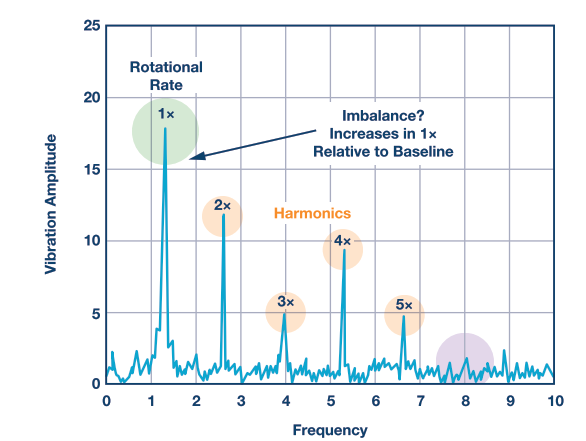
\includegraphics[scale=.25]{../referencial/img/imbalance_analog_p2.png}
					\caption{Indicação espectral de desbalanceamento na velocidade. \newline
					Fonte: \citeonline{Sopcik2019}.} 
					\label{fig:imbalance_analog_p2}
				\end{center}
			\end{figure}
	 	\end{column}
	 \end{columns}
\end{frame}

%%%%%%%%%%%%%%%%%%%%%%%%%%%%%%%%%%%

\begin{frame}{Referencial Teórico - Análise de Corrente Elétrica}
	\begin{columns}
    	\begin{column}{0.50\textwidth}
			\begin{figure}[HT]
				\begin{center}
					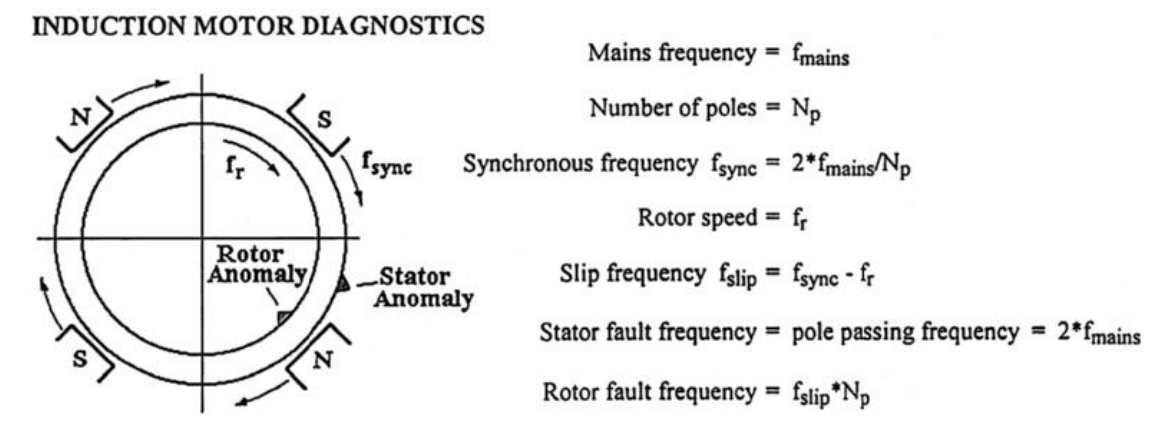
\includegraphics[scale=.35]{../referencial/img/fault_freq_randall_p55.png}
					\caption{Ilustração com as frequências associadas às falhas em rotores ou estatores de motores elétricos. \newline
					Fonte: \citeonline{Wu2013}.} 
					\label{fig:fault_freq_randall_p55}
				\end{center}
			\end{figure}
     	\end{column}
		
		\begin{column}{0.5\textwidth}
			\begin{figure}[HT]
				\begin{center}
					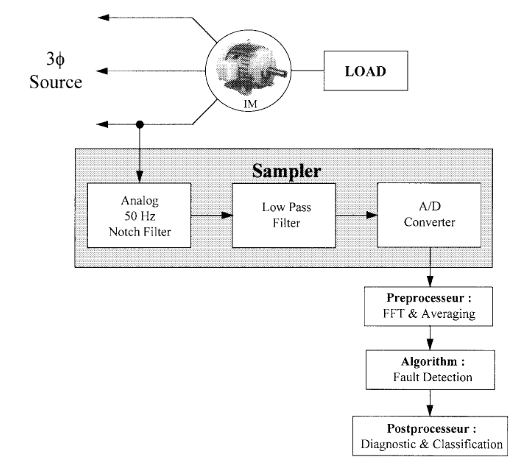
\includegraphics[scale=.5]{../referencial/img/current_benbouzid_p3.png}
					\caption{Indicação espectral de desbalanceamento na velocidade. \newline
					Fonte: \citeonline{El1999}.} 
					\label{fig:current_benbouzid_p3}
				\end{center}
			\end{figure}
	 	\end{column}
	 \end{columns}
\end{frame}

%%%%%%%%%%%%%%%%%%%%%%%%%%%%%%%%%%%

\begin{frame}{Referencial Teórico - Técnicas Modernas de Processamento de Sinais}
	\begin{columns}
    	\begin{column}{0.50\textwidth}
			\begin{figure}[HT]
				\begin{center}
					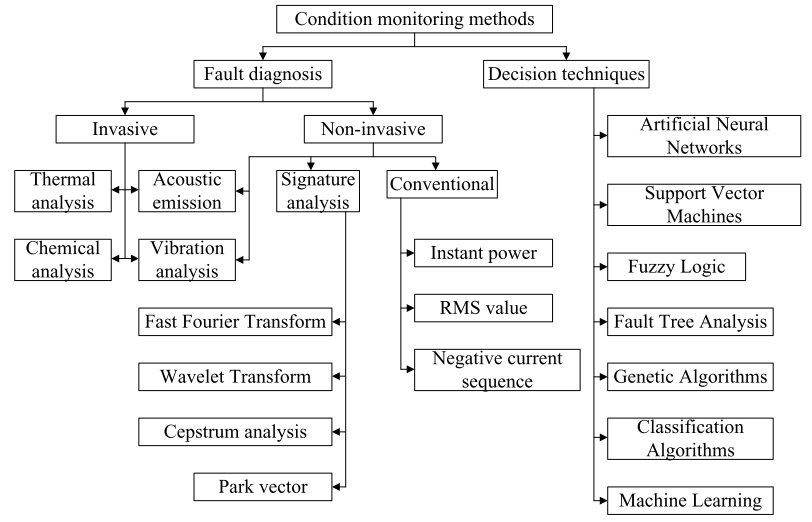
\includegraphics[scale=.5]{../referencial/img/monitoring_methods_rilski_p78.png}
					\caption{Árvore de métodos de monitoramento de falhas em motores elétricos. \newline
					Fonte: \citeonline{Gorbounov2018}.} 
					\label{fig:monitoring_methods_rilski_p78}
				\end{center}
			\end{figure}
     	\end{column}
		
		\begin{column}{0.5\textwidth}
			\begin{itemize}
				\item FFT 
			\end{itemize}			
	 	\end{column}
	 \end{columns}
\end{frame}
%%%%%%%%%%%%%%%%%%%%%%%%%%%%%%%%%%%

\section{Metodologia}
\begin{frame}{Metodologia - }
	\begin{columns}
    	\begin{column}{0.50\textwidth}
			\begin{figure}[HT]
				\begin{center}
				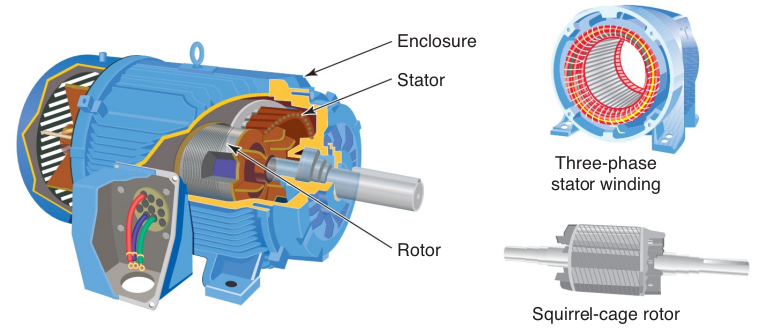
\includegraphics[scale=.25]{../referencial/img/ind_motor_petruzella_p115.png}
				\caption{Motor elétrico de indução tipo gaiola de esquilo. \newline
				Fonte: \citeonline{Petruzella1911}.}
				\label{fig:ind_motor_petruzella_p115}
				\end{center}
			\end{figure}
     	\end{column}
		
		\begin{column}{0.5\textwidth}
			\begin{itemize}
				\item infos
			\end{itemize}
	 	\end{column}
	 \end{columns}
\end{frame}

%%%%%%%%%%%%%%%%%%%%%%%%%%%%%%%%%%%

\section{Análise dos Resultados}
\begin{frame}{Análise dos Resultados - }
	\begin{columns}
    	\begin{column}{0.50\textwidth}
			\begin{figure}[HT]
				\begin{center}
				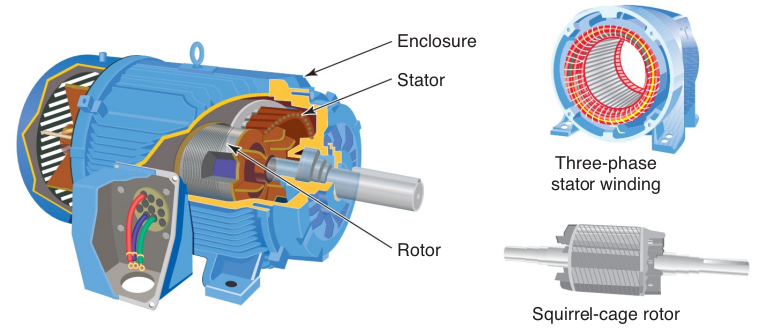
\includegraphics[scale=.25]{../referencial/img/ind_motor_petruzella_p115.png}
				\caption{Motor elétrico de indução tipo gaiola de esquilo. \newline
				Fonte: \citeonline{Petruzella1911}.}
				\label{fig:ind_motor_petruzella_p115}
				\end{center}
			\end{figure}
     	\end{column}
		
		\begin{column}{0.5\textwidth}
			\begin{itemize}
				\item infos
			\end{itemize}
	 	\end{column}
	 \end{columns}
\end{frame}

%%%%%%%%%%%%%%%%%%%%%%%%%%%%%%%%%%%

\section{Conclusão}
	\begin{frame}{Conclusão}
    \begin{itemize}
        	\justifying
			\item Perceptível influência da vibração dos motores na resposta do movimento de rotação do sumulador.
			\item Necessidade de melhorias no sistema inercial.
			\item Possibilidade de se empregar técnicas modernas em controle, onde uma RNA aprendeu o comportamento de dinâmica de um simulador de satélites.
		\end{itemize}
\end{frame}

%%%%%%%%%%%%%%%%%%%%%%%%%%%%%%%%%%%

\begin{frame}{Conclusão - Trabalhos futuros}
    \begin{itemize}
        \justifying
		\item Substituição do inercial simples por um absoluto com processamento integrado. 
		\item Criação de uma interface gráfica para o usuário.
		\item Essa interface será didática, auxiliando o ensino da teoria de controle.  
		\item Disponibilizar todos os códigos fonte no GitHub e Bitbucket.
		\end{itemize}
\end{frame}

%%%%%%%%%%%%%%%%%%%%%%%%%%%%%%%%%%%

\section{Referências Bibliográficas}
\begin{frame}{Referências Bibliográficas}
	\bibliography{../referencial/references}
\end{frame}

%%%%%%%%%%%%%%%%%%%%%%%%%%%%%%%%%%%

\begin{frame}{Agradecimentos}
		\begin{center}
			{\Huge Obrigado pela Atenção!}
		\end{center}
\end{frame}

\end{document}